% -----------------------------------------------
% Template for ISMIR Papers
% 2015 version, based on previous ISMIR templates
% -----------------------------------------------

\documentclass{article}
\usepackage{ismir,amsmath,cite}
\usepackage{graphicx}
\usepackage{color}

% Title.
% ------
\title{Paper Template For ISMIR \conferenceyear}


% Single address
% To use with only one author or several with the same address
% ---------------
%\oneauthor
% {Names should be omitted for double-blind reviewing}
% {Affiliations should be omitted for double-blind reviewing}

% Two addresses
% --------------
%\twoauthors
%  {First author} {School \\ Department}
%  {Second author} {Company \\ Address}

% Three addresses
% --------------
\threeauthors
  {Jose Pedro de Santana Neto} {University of Brasilia - FGA\\ {\tt 1jpsneto@gmail.com}}
  {Henrique Gomes de Moura} {University of Brasilia - FGA\\ {\tt hgmoura@yahoo.com}}
  {Fernando William Cruz} {University of Brasilia - FGA\\ {\tt fwcruz@unb.br}}

% Four addresses
% --------------
%\fourauthors
%  {First author} {Affiliation1 \\ {\tt author1@ismir.edu}}
%  {Second author}{Affiliation2 \\ {\tt author2@ismir.edu}}
%  {Third author} {Affiliation3 \\ {\tt author3@ismir.edu}}
%  {Fourth author} {Affiliation4 \\ {\tt author4@ismir.edu}}

\begin{document}
%
\maketitle
%
\begin{abstract}

Neste trabalho eh apresentado um metodo alternativo e eficiente para a construcao de chroma feature ou Pitch Class Profile (PCP). O Chroma Convolution Method (CCM), que eh uma operacao essencialmente no dominio temporal, possui caracteristicas particulares que otimizam a distincao de notas e timbres de instrumentos musicais. Para a demonstracao da eficacia desse metodo, foram feitos dois experimentos comparativos com o metodo tradicional DFT ou STFT. Os experimentos mostraram que o CCM eh mais eficaz em identificacao das notas, como tambem, possui a capacidade de distincao de notas de diferentes instrumentos musicais tocados ao mesmo tempo.  

\end{abstract}
%
\section{Introduction}\label{sec:introduction}

% 1- problema

	O processo de extracao de caracteristicas cromaticas eh um problema constante em solucoes de transcricao automatica de musica. Basicamente este processo consiste em obter o espectro de frequencias do sinal de audio, calcular o nivel de energia de cada nota corresponte a frequencia de cada uma das 12 notas musicais que compoem a escala temperada. Tradicionalmente usa-se a transformada de fourier para tal tarefa desde meados de 1999 com Fujishima \cite{fujishima1999realtime} e, desde entao, varios esforcos sao empreendidos para otimizar o Pitch Class Profile (PCP) construido via transformada discreta de fourier (DFT) .

% 2- Estudos que abordaram o problema
	Varios estudos abordaram o problema de construcao de chroma feature em musicas. Tais estudos construiram solucoes embasadas em DFT ou STFT (Short Fast Fourier Transform) para idenficacao de melodias: \cite{muto2002transcription}, \cite{al2008time}, \cite{barbancho2009transcription}, \cite{gomez2004automatic}, \cite{tangmelody}, \cite{eggink2004extracting} e \cite{jo2010melody}, esse ultimo usando filtros particula para otimizacao. Ha tambem estudos de solucoes de chroma feature com foco em transcricao automcatica de acordes via DFT:
	\cite{harte2009automatic}, \cite{khadkevich2011time}, \cite{harte2010towards}, \cite{peeters2006chroma}, \cite{cho2010exploring} \cite{lee2006automatic}, \cite{de2012improving}, \cite{boulanger2013audio}, \cite{chen2012chord} e \cite{hrybyk2010combined}.

% 3- deficiencias nos estudos
	Tais estudos focaram solucoes adapatadas em DFT e pouco se tem outras alternativas para caracterizacao de notas. Ha tambem varias limitacoes citadas da DFT em trabalhos como o de Harte\cite{harte2010towards}. O estudo de Mauch\cite{mauch2010approximate} por exemplo foca a aplicacao de NNLS para aumentar a identificacao de notas e o trabalho \cite{wakefield1999mathematical} foca a modelagem matematica	para a representacao da distribuicao das notas em suas frequencias. Porem ha ainda a carencia de metodos alternativos em relacao a DFT para a construcao de chroma feature.

% 4- importancia do estudo para o publico
	O presente trabalho foca a apresentacao de um metodo alternativo e mais eficiente que a DFT, no que tange a identificacao das notas, para a construcao do chroma feature. A alternativa Chroma Convolution Method (CCM), que eh uma operacao essencialmente de dominio temporal, possui caracteristicas particulares que otimizam a distincao de notas e timbres de instrumentos musicais. O CCM pode ser usado no lugar da DFT ou STFT para extrair sons polifonicos com mais acuracia, identificando notas de diferentes instrumentos musicais.

	Este paper esta organizado da seguinte forma: Section 2 descreve o uso, aspectos gerais e limitacoes da DFT; Section 3 apresenta a conceituacao do metodo proposto, caracteristicas e processo de construcao do chroma feature usando o CCM; Section 4 apresenta dois experimentos de comparacao dos metodos DFT e CCM; Section 5 delimita discussoes sobre os resultados da eficacia do CCM; Section 6 apresenta conclusoes e trabalhos futuros.

\section{Discrete Fourier Transform (DFT)}\label{sec:sfft}

	Chroma feature ou pitch class profile (PCP) tem sido usado quase exclusivamente como um front-end para o
	reconhecimento de acordes ou extracção de melodias de audio gravado. Fujishima \cite{fujishima1999realtime} desenvolveu um sistema de transcricao automatica de acordes em tempo real, onde ele deriva um chroma feature de 12 dimensoes a partir do DFT do sinal de audio. Desde entao a transformada discreta de fourier (DFT ou  FFT) tem sido muito utilizada para a construcao das caracteristicas cromaticas (chroma feature) do audio. A funcao dessa transformada eh traduzir informacoes que estao em dominio temporal para dominio frequencial de tal forma a projetar, em bases ortonormais, o valor de cada componente senoidal presente no sinal tratado. Essa projecao se da pelo somatorio do produto interno das senoides (exponenciais complexas) pelo sinal \cite{vaidyanathan1993multirate}.

	Visto que essa transformada somente oferece informacoes em termos de frequencias, surgiu-se a necessidade de adapta-la para a visualizacao das variacoes das frequencias ao longo do tempo. Essa adaptacao se denomina short time fourier transform (STFT) \cite{cohen1995time}. Esse processo de janelamento se resume a dividir o sinal em partes, para serem analisadas individualmente no domínio da frequencia, ou seja, a cada instante de tempo referente a cada trecho eh possivel obter uma analise frequencial.

	Porem essa tecnica possui as seguintes limitacoes:
	\begin{itemize}
		\item surgimento de frequencias fantasmas (alising) que podem dificultar a identificacao das notas musicais que foram verdadeiramente tocadas;
		\item problemas de vazamento gerados pelo truncamento do sinal, podendo gerar frequencias que dificultam a visualizacao do espectro (leakage);
		\item dificuldades na determinacao do tamanho da janela pois trata-se de um parametro de amostragem que pode limitar a banda de frequencia a ser analisada.
	\end{itemize}

	Observa-se que as limitacoes apresentadas sao, em grande parte, oriundas do processamento digital de sinais necessario para a constituicao do espectro de frequencias. Deste modo, surge a necessidade de se pesquisar alternativas para o problema de construcao do chroma feature no dominio do tempo, preservando assim as caracteristicas originais do sinal de audio.

\section{Chroma Convolution Method (CCM)}\label{sec:ccm}

	O chroma convolution method (CCM) objetiva a projecao dos trechos do sinal sobre cada um dos sinais das notas musicais procuradas. Observa-se que quando o trecho do sinal eh projetado sobre o sinal de uma nota musical, atraves da convolucao, esta nota eh amplificada e as demais sao suprimidas.

	Seja uma nota musical formada a partir de uma senoide monocromatica. Quando esse sinal eh convoluido com um trecho de sinal de audio eh possivel extrair como resultado o nivel de energia relacionado a esta frequencia. Tal energia eh mensurada a partir da seguinte equacao \eqnref{ccm_equation}:

	\begin{equation}\label{ccm_equation}
		E = \sum [f(x)*g(x)]^{2}
	\end{equation}

	Neste contexto as caracteristicas cromaticas (chroma feature) foram construidas a partir dos seguintes procedimentos:
	\begin{enumerate}
		\item dividiu-se o audio a ser analisado em sinais com duracao pre-determinada;
		\item funcoes senoidais monocromaticas foram utilizadas para construir notas musicais no dominio do tempo, correspondendo a escala cromatica musical; 
		\item convoluiu-se cada parte do sinal de audio com as notas musicais;
		\item a energia da convolucao foi extraida a partir da equacao \eqnref{ccm_equation};
		\item por fim cada energia foi somada com suas respectivas oitavas, originando o chroma feature, esquematicamente apresentado em \figref{fig:chroma_feature}.
	\end{enumerate}

	\newpage
	\begin{figure}[h]
		 \centerline{\framebox{
		 \includegraphics[width=\columnwidth, height=6cm]{figs/chroma_feature.png}}}
		 \caption{Schematic representation of the chroma feature. On this chart, a full chromatic scale starting from A up to G\#.}
		 \label{fig:chroma_feature}
		\end{figure}

	A \figref{fig:schematic} representa uma visao esquematica do procedimento descrito. Ao final do processo as caracteristicas cromaticas (chroma feature) podem ser visualizadas a partir de um espectrograma de 12 dimensoes.

	\begin{figure}[h]
	 \centerline{\framebox{
	 \includegraphics[width=\columnwidth]{figs/schematic.png}}}
	 \caption{Schematic of process to build chroma feature using CCM.}
	 \label{fig:schematic}
	\end{figure}


\section{Experiments and Results}

	Com o intuito de demonstrar a eficacia do CCM em relacao ao tradicional metodo STFT\cite{LabROSA}, no que diz respeito identificacao das notas tocadas a partir de suas caracteristicas cromaticas (chroma feature), foram realizados 2 experimentos usando a linguagem de programacao MATLAB. Como entrada de dados usou-se sinais de audio gravados por instrumentos musicais reais\footnote{Code and files available in https://github.com/josepedro/ismir\_article.}. 

	\newpage
	\subsection{Experiment 1: Identification of Musical Notes}

	O primeiro experimento se trata de identificacao de notas musicais numa melodia de piano. Tais notas foram tocadas segundo a \figref{fig:1-notes}.

	\begin{figure}[h]
	 \centerline{\framebox{
	 \includegraphics[width=\columnwidth]{figs/1-notes.png}}}
	 \caption{Recorded notes played on piano.}
	 \label{fig:1-notes}
	\end{figure}

	Utilizou-se convolucao com 96 tons puros de diferentes frequencias para gerar o chroma feature. As janelas de ambas as propostas foram configuradas no tamanho de 0.120 segundos e a taxa de amostragem do audio foi de 44.1 kHz.

	\subsubsection{STFT Results}
	Segue chroma feature encontrado utilizando o metodo tradicional da STFT em \figref{fig:1-ssft}. Observa-se que a escala cromatica foi identificada, porem com erros em relacao ao momento exato em que as notas foram tocadas. Nota-se, por exemplo, que uma nota E foi identificada no comeco quando na verdade deveria ter sido identificada nos instantes proximos de 7 segundos.

	
	\begin{figure}[h]
	 \centerline{\framebox{
	 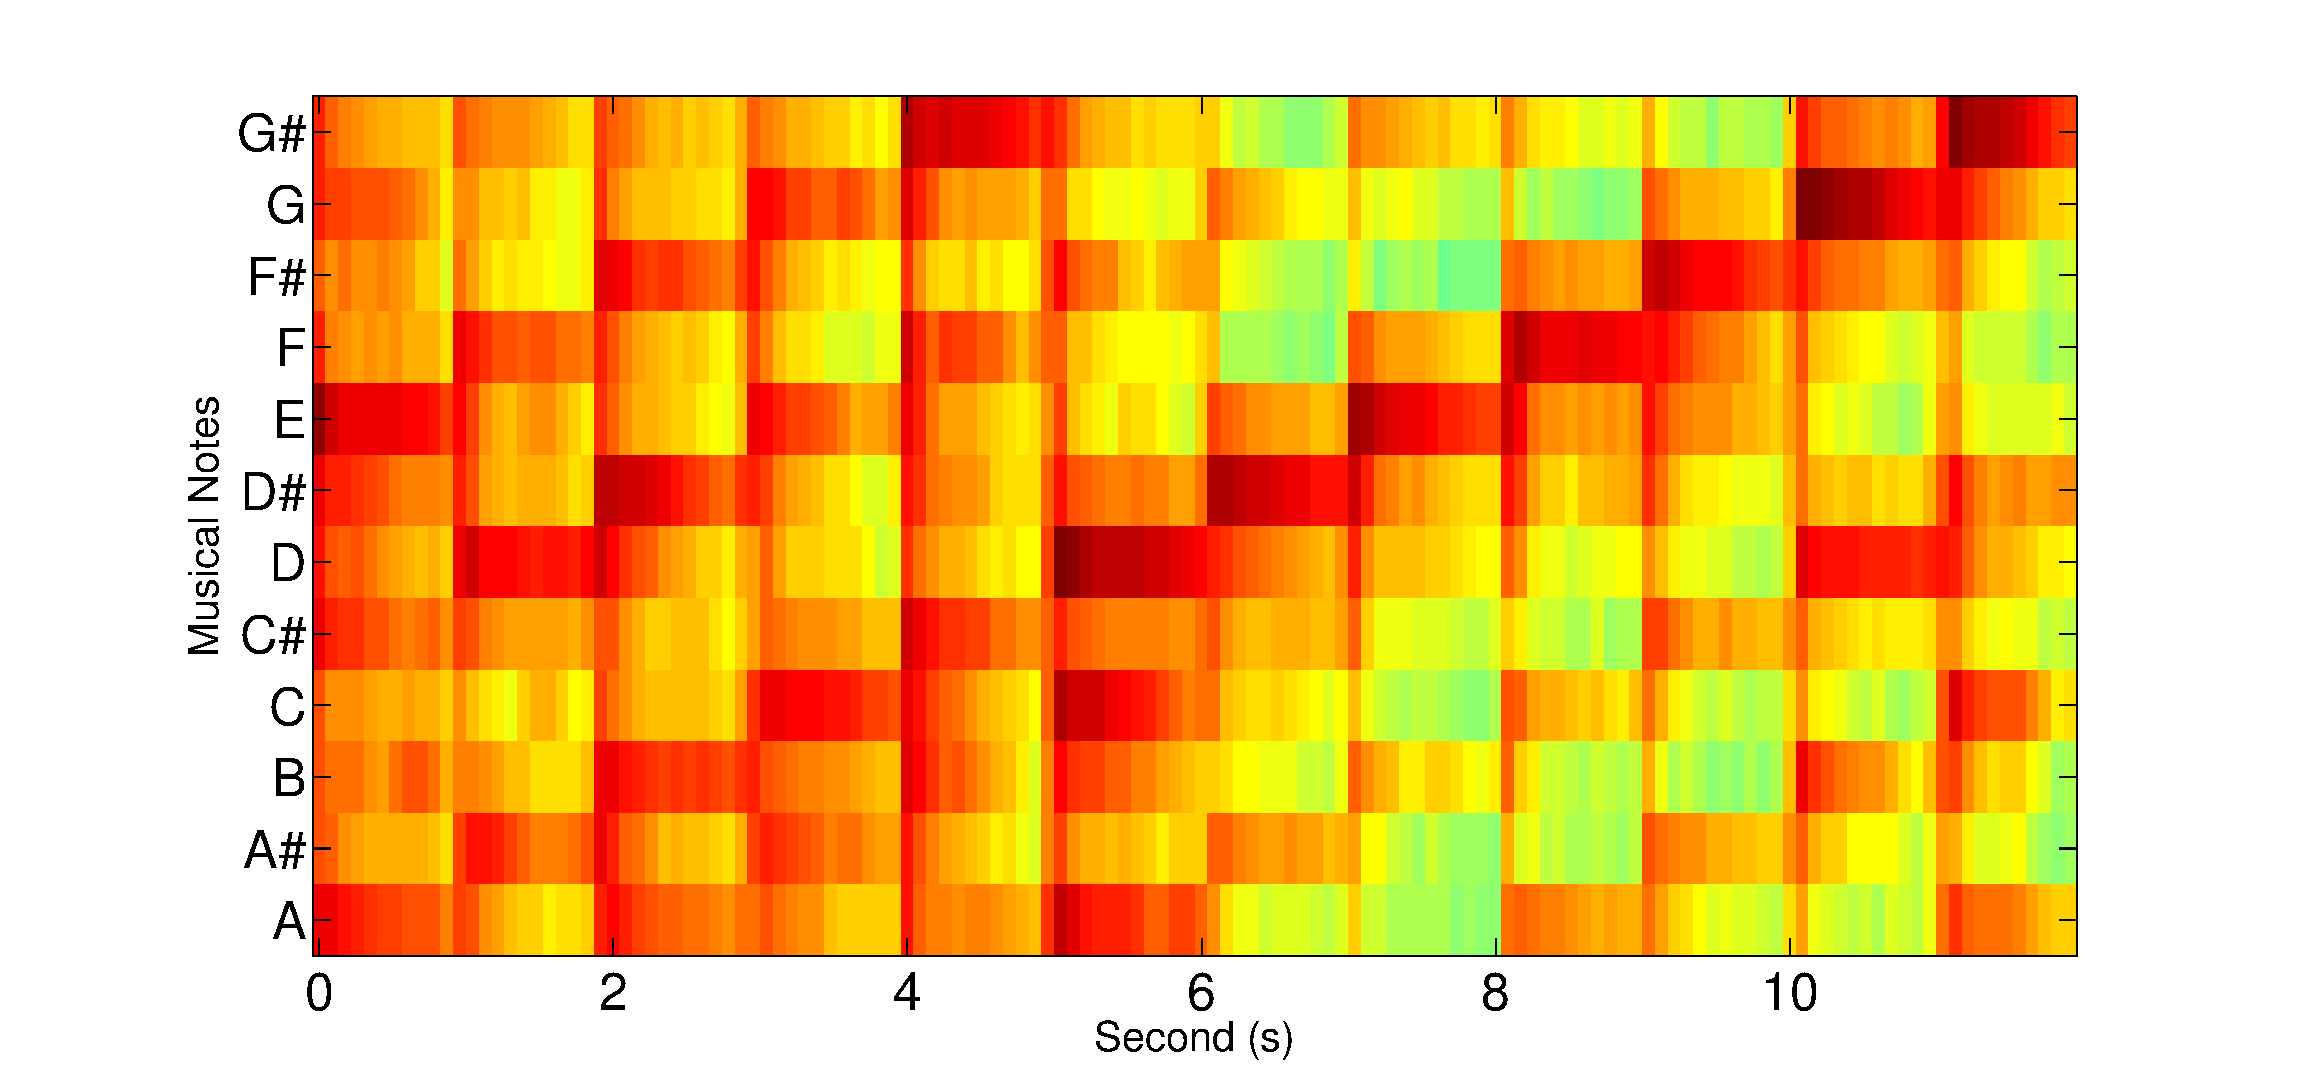
\includegraphics[width=\columnwidth, height=6cm]{figs/1-sfft.eps}}}
	 \caption{Obtained chroma feature by using the STFT method.}
	 \label{fig:1-ssft}
	\end{figure}	

	
	Foi tambem feito uma analise de eficiencia das notas gravadas no audio com a sequencia de notas identificas no chroma feature. As notas identificadas foram selecionadas atraves da maior intensidade em cada instante de tempo. A \tabref{tab:table-1-sfft} representa as notas tocadas e as que foram identificadas no chroma feature. Houveram 9 de 14 notas tocadas em instantes corretos, ou seja, 64.3\% de fidelidade com a melodia original.

	\newpage

	\begin{table}[h]
	 \begin{center}
	 \begin{tabular}{|l|l|}
	  \hline
	  Played Notes & Identified Notes \\
	  \hline
	  A  & E \\
	  A\#  & D \\
	  A\#  & D\# \\
	  B  & B \\
	  B\#  & E \\
	  C  & D \\
	  C\#  & G\# \\
	  D  & D \\
	  D\#  & D\# \\
	  E  & E \\
	  F  & F \\
	  F\#  & F\# \\
	  G  & G \\
	  G\#  & G\# \\
	  \hline
	 \end{tabular}
	\end{center}
	 \caption{Comparison between played and identified notes by the STFT method.}
	 \label{tab:table-1-sfft}
	\end{table}

	


	\subsubsection{CCM Results}
	Segue chroma feature encontrado utilizando o CCM em \figref{fig:1-ccm}.
	
	\begin{figure}[h]
	 \centerline{\framebox{
	 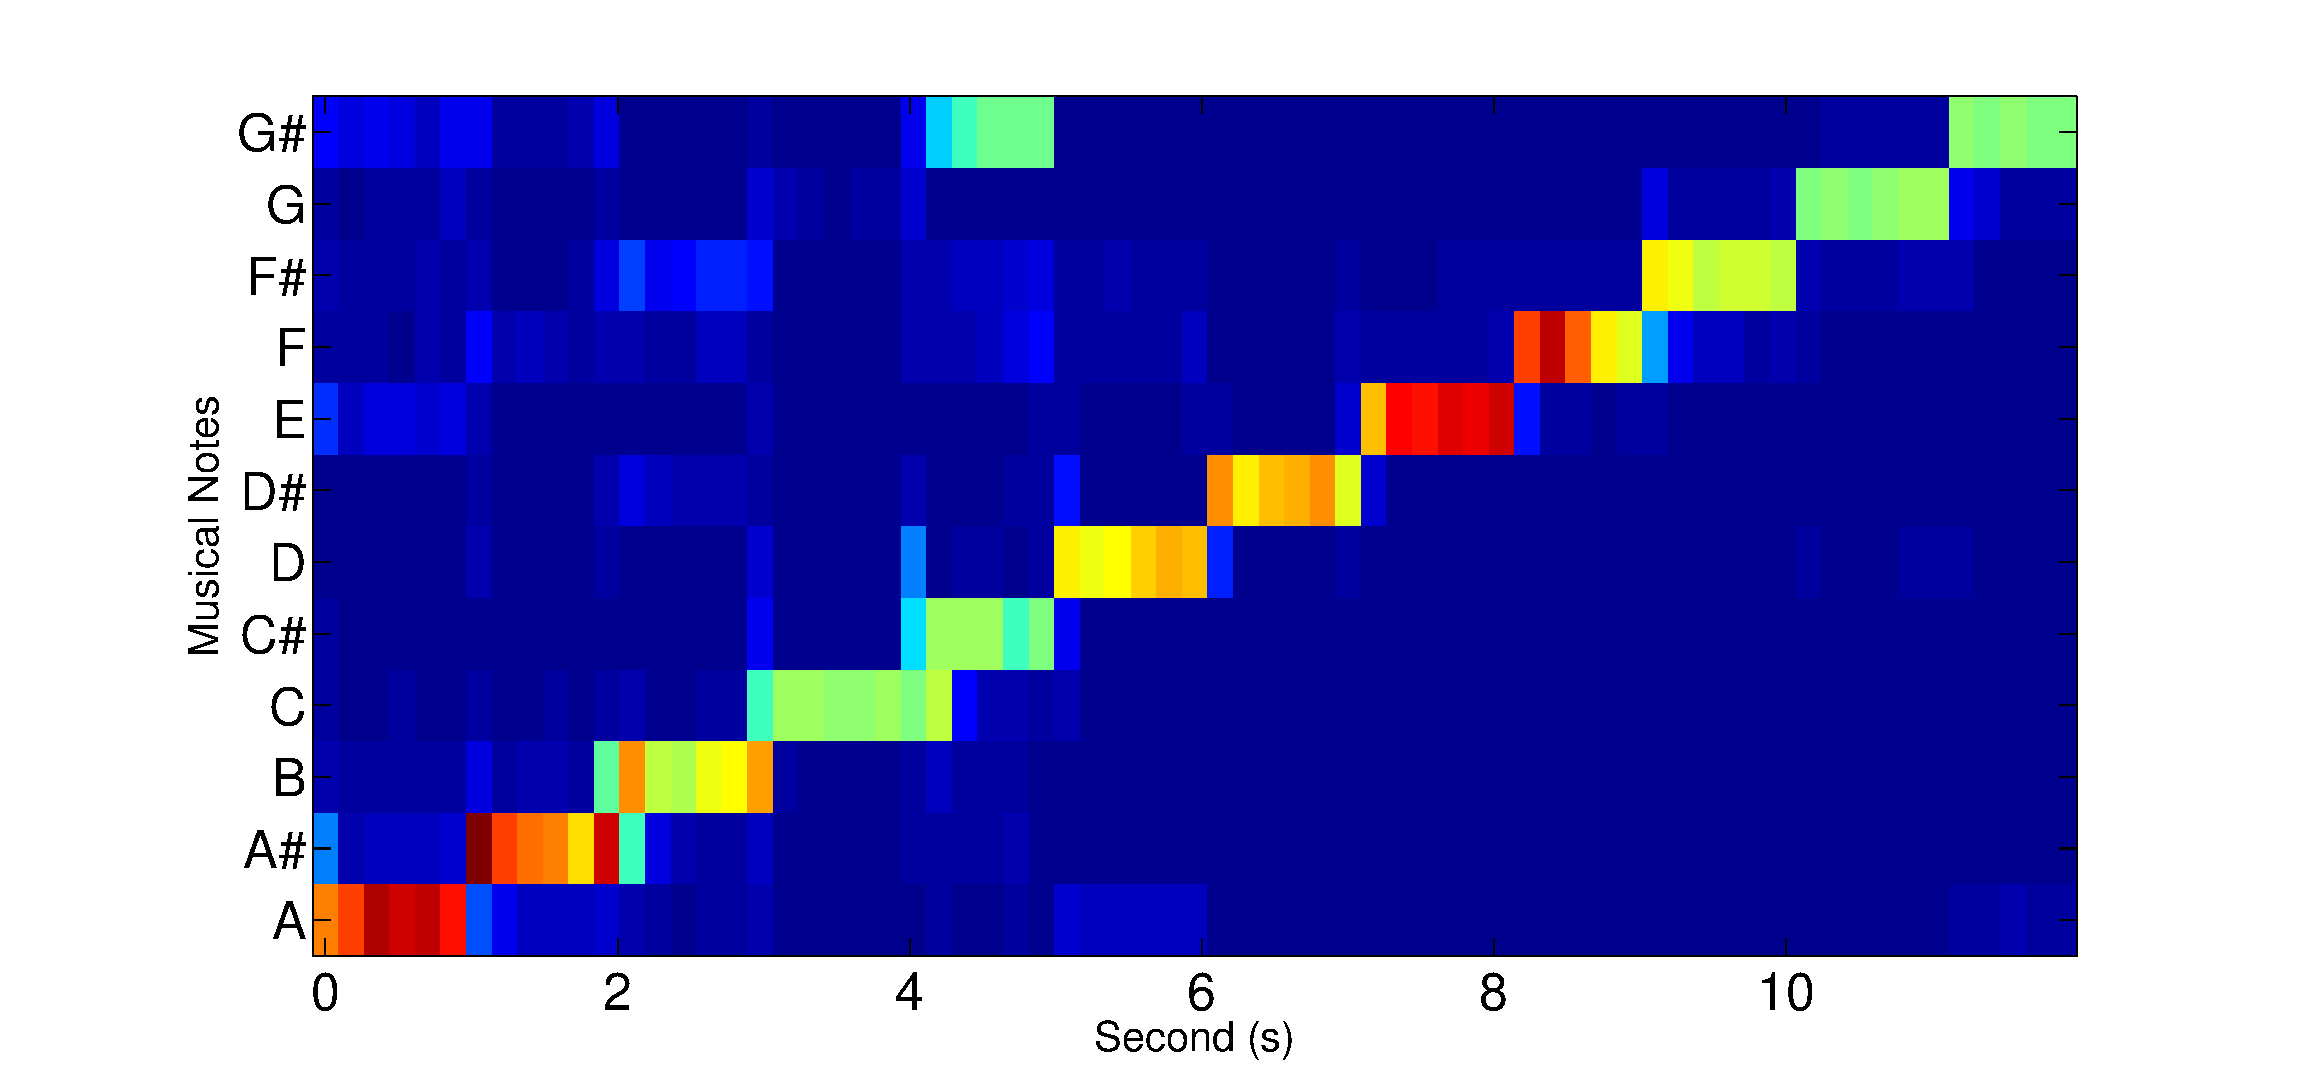
\includegraphics[width=\columnwidth, height=6cm]{figs/1-ccm.eps}}}
	 \caption{Obtained chroma feature by using the Chroma Convolution method.}
	 \label{fig:1-ccm}
	\end{figure}	


	Observa-se na figura \figref{fig:1-ccm} que a melodia apresentou uma maior clareza. Uma tabela comparativa das notas tocadas e identificadas foi feita tambem atraves da estrategia dos maximos. Em vista dos resultados de \tabref{tab:table-1-ccm}, houve 13 de 14 notas tocadas em instantes corretos, ou seja, 92.9\% de fidelidade com a melodia original.

	\newpage

	\begin{table}[h]
	 \begin{center}
	 \begin{tabular}{|l|l|}
	  \hline
	  Played Notes & Identified Notes \\
	  \hline
	  A  & A \\
	  A\#  & A\# \\
	  B  & B \\
	  C  & C \\
	  C\#  & C\# \\
	  C\#  & G\# \\
	  C\#  & C\# \\
	  D  & D \\
	  D\#  & D\# \\
	  E  & E \\
	  F  & F \\
	  F\#  & F\# \\
	  G  & G \\
	  G\#  & G\# \\
	  \hline
	 \end{tabular}
	\end{center}
	 \caption{Comparison between played and identified notes by the Chroma Convolution Method.}
	 \label{tab:table-1-ccm}
	\end{table}


	\subsection{Experiment 2: Identification of Musical Notes of Different Instruments}

	O segundo experimento diz respeito a identificação de notas musicais de diferentes instrumentos. Para tal foram tocadas as seguintes melodias no piano e violao juntas representadas em \figref{fig:2-melodias}.

	\begin{figure}[h]
	 \centerline{\framebox{
	 \includegraphics[width=\columnwidth]{figs/1-notes.png}}}
	 \centerline{\framebox{
	 \includegraphics[width=\columnwidth]{figs/2-notes-violao.png}}}
	 \centerline{\framebox{
	 \includegraphics[width=\columnwidth]{figs/2-notes-violao-piano.png}}}
	 \caption{The first sheet music is only piano, the second sheet music is only acoustic guitar and the third sheet music is the both together.}
	 \label{fig:2-melodias}
	\end{figure}

Utilizou-se convolucao com 12 tons de violao e 12 tons de piano de diferentes frequencias gerando dois chroma feature respectivamente, um para cada instrumento. As janelas de ambas as propostas foram configuradas no tamanho de 0.120 segundos e a taxa de amostragem do audio foi de 44.1 kHz.

	\subsubsection{STFT Results}
	Segue chroma feature encontrado utilizando o metodo tradicional da STFT em \figref{fig:2-ssft}. Observa-se nessa figura que a escala cromatica do piano foi parcialmente identificada. As notas do violao sao praticamente imperceptiveis.
	\newpage
	
	\begin{figure}[h]
	 \centerline{\framebox{
	 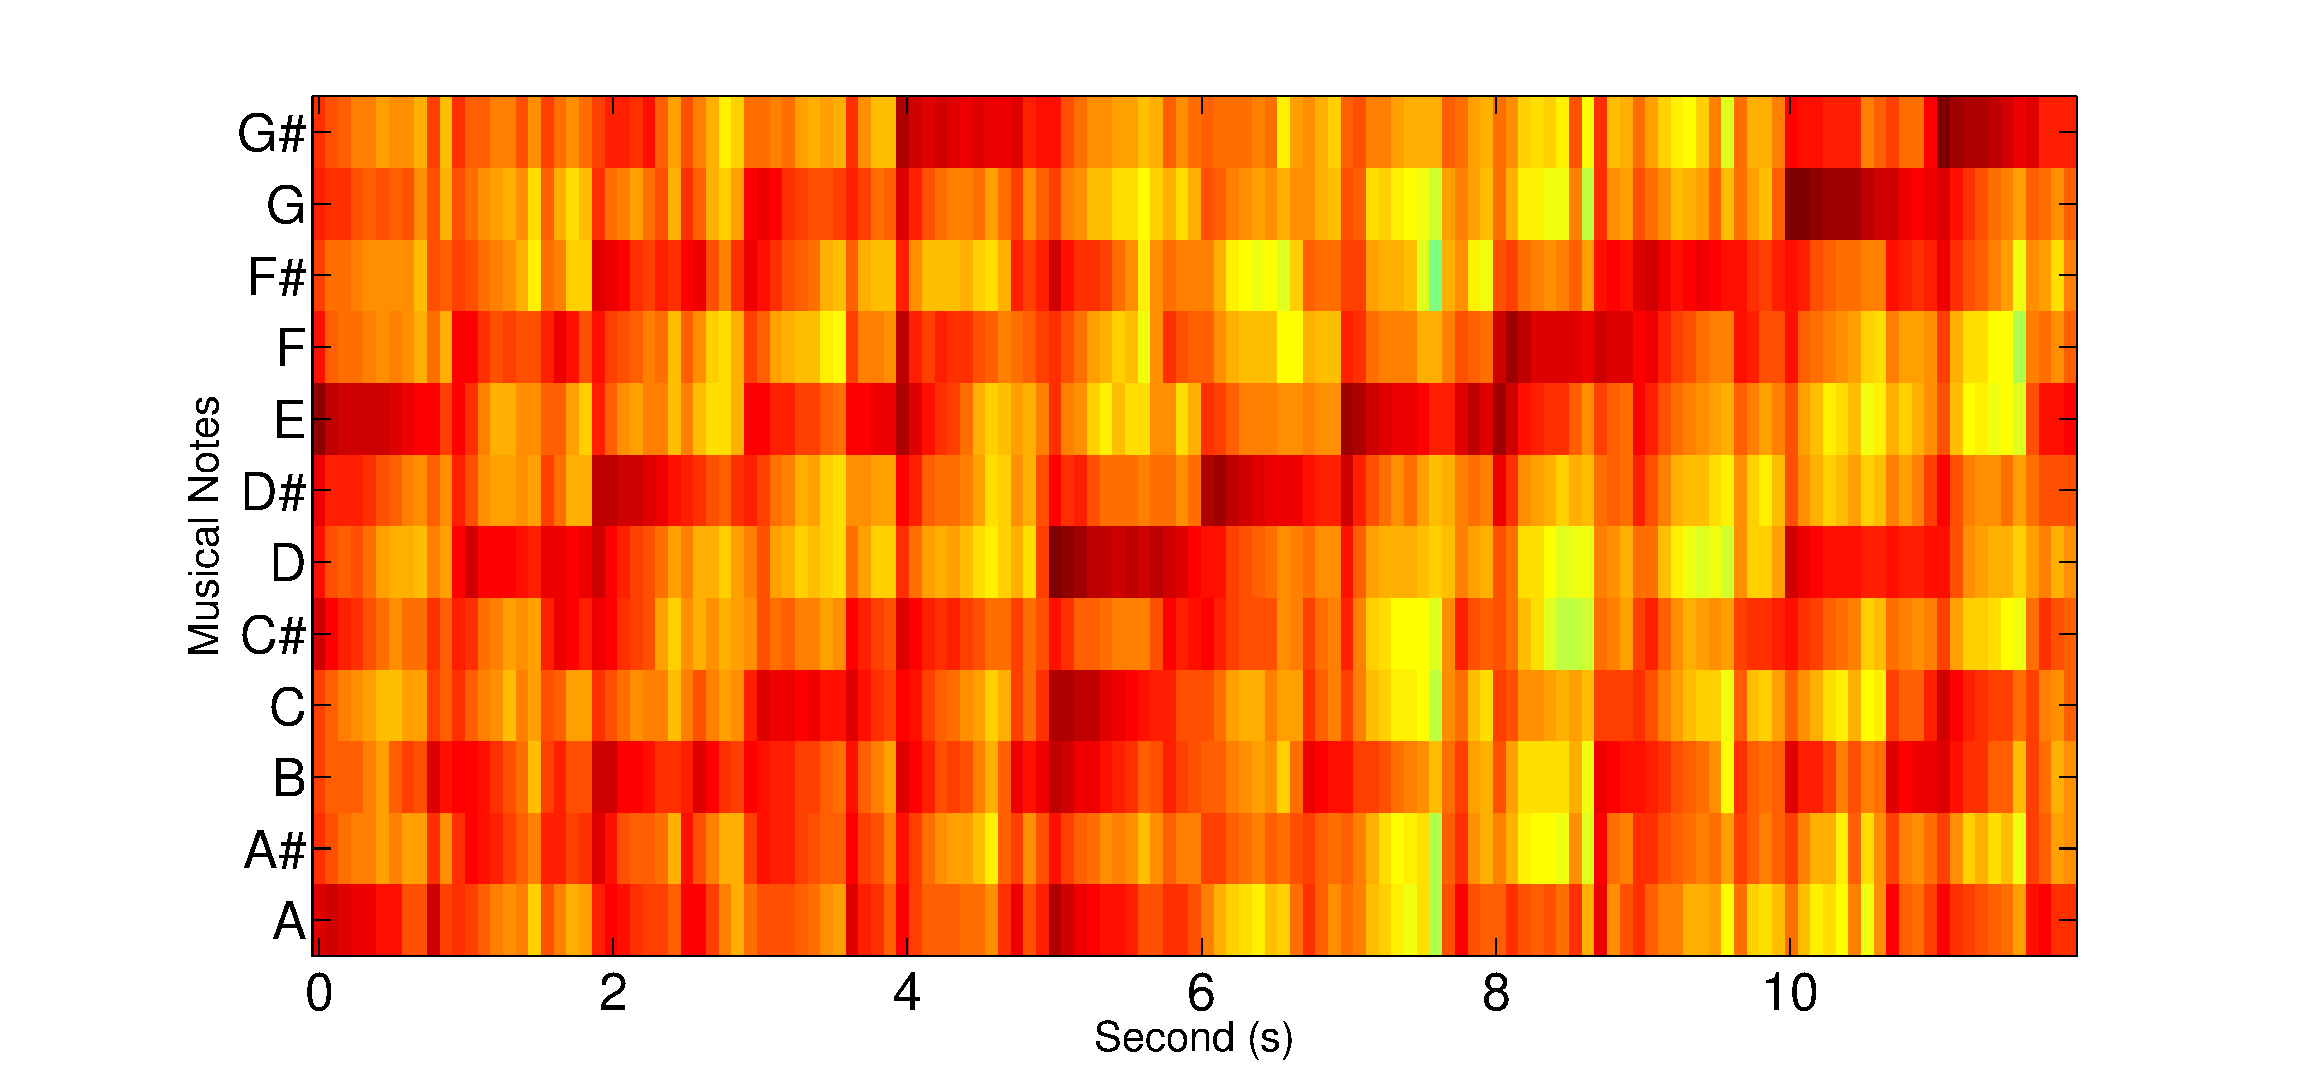
\includegraphics[width=\columnwidth, height=6cm]{figs/2-sfft.eps}}}
	 \caption{Chroma feature of audio using STFT.}
	 \label{fig:2-ssft}
	\end{figure}	

	Foi tambem feito uma analise de eficiencia das notas gravadas dos dois instrumentos com a sequencia de notas identificadas no chroma feature, usando a maior intensidade em cada instante de tempo. Segue tabela comparativa em \tabref{tab:table-2-sfft}.

	\begin{table}[h]
	 \begin{center}
	 	\centerline{
	 \includegraphics[width=\columnwidth,height=9cm]{figs/tabela_2.png}}
	 \end{center}
	 \caption{Comparison between played notes of piano, acoustic guitar and identified by the STFT method.}
	 \label{tab:table-2-sfft}
	\end{table}


	\newpage

	Primeiramente eh importante ressaltar que nao eh possivel obter um chroma feature para cada instrumento usando o metodo STFT. Deste modo, utilizando a estrategia da maxima intensidade a cada instante de tempo, so foi possivel obter um valor de eficiencia global em torno de 38.7\%, ou seja, a cada instante de tempo uma nota das duas notas tocadas pelos instrumentos, piano e violao, deveria ter sido identificada. Os resultados dessa analise se encontram em \tabref{tab:table-2-sfft}.

%-------------------------------------------------------------------
	\subsubsection{CCM Results}
	Segue chroma feature encontrado utilizando o CCM de tons de piano:
	
	\begin{figure}[h]
	 \centerline{\framebox{
	 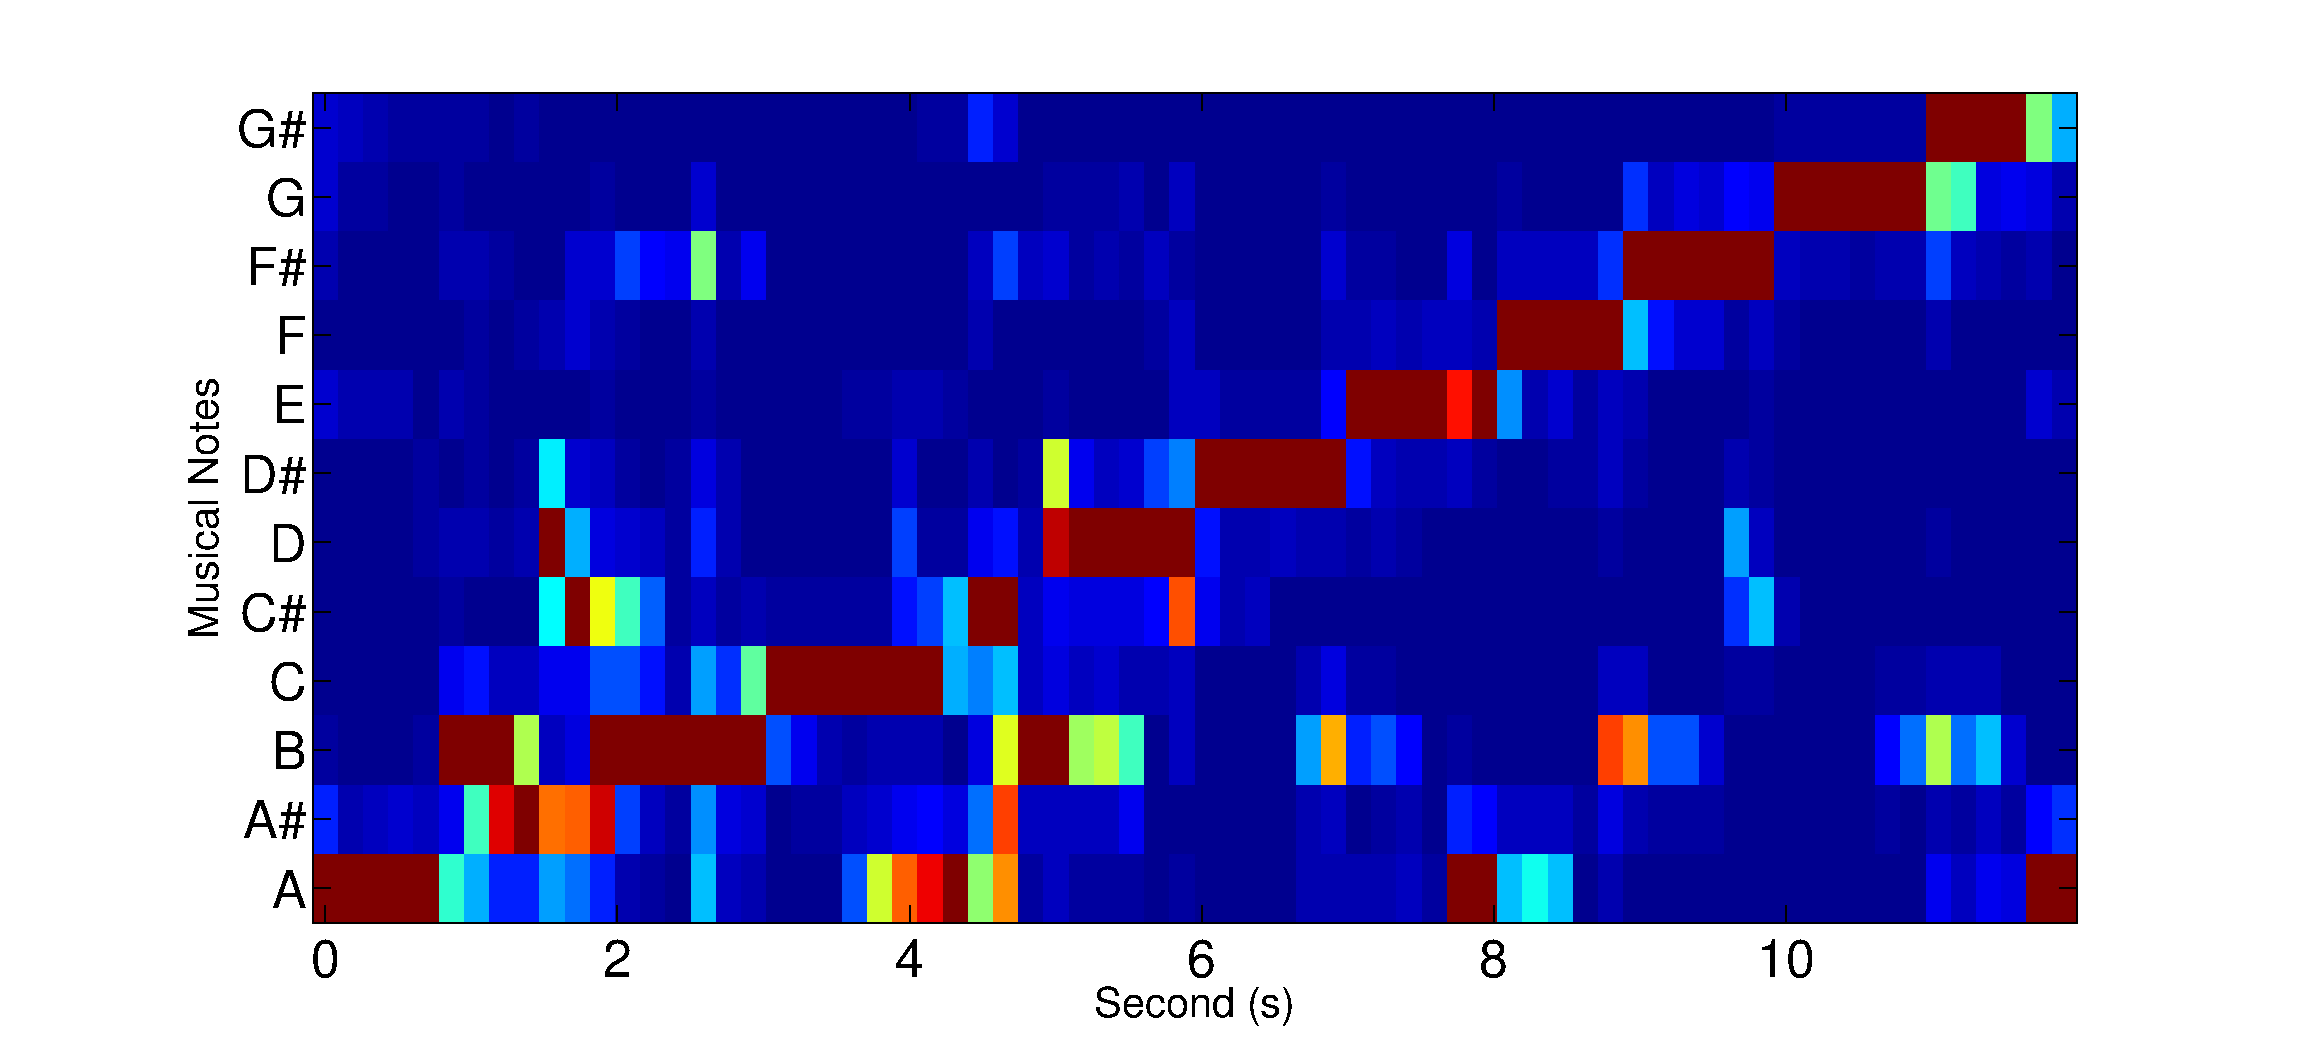
\includegraphics[width=\columnwidth, height=6cm]{figs/2-ccm-piano.eps}}}
	 \caption{Chroma feature of audio using CCM of piano tones.}
	 \label{fig:2-ccm-piano}
	\end{figure}	

	Observa-se na figura \figref{fig:2-ccm-piano} que a melodia executada no piano foi identificada com maior clareza. Sao visiveis tambem algumas notas executadas no violao. Uma tabela comparativa das notas tocadas identificadas foi feita tambem atraves da estrategia dos maximos. Em vista dos resultados de \tabref{tab:table-2-ccm-piano}, houveram 13 de 18 notas de piano em instantes corretos, ou seja, 72.2\% de fidelidade com a melodia original. Quanto ao violao, houveram 5 de 18 notas em instantes corretos, ocasionando em 27.7\%. Tal resultado mostra que neste experimento o CCM amplificou as notas executadas pelo piano e suprimiu as notas executadas pelo violao.

	\begin{table}[h]
	 \begin{center}
	 \begin{tabular}{|l|l|l|}
	  \hline
	  Piano & Acoustic Guitar & Identified Notes \\
	  \hline
		A	& A	& A \\
		A	&    B	&    B \\
		A\#	&    B	&    A\# \\
		A\#	&    B	&    C\# \\
		A\#	&    C\#	&    A\# \\
		B	&    B	&    B \\
		C	&    A	&    C \\
		C\#	&    A	&    A \\
		C\#	&    B	&    C\# \\
		D	&    B	&    B \\
		D	&    C\#	&    D \\
		D\#	&    B	&    D\# \\
		E	&    A	&    E \\
		F	&    B	&    F \\
		F\#	&    C\#	&    F\# \\
		G	&    B	&    G \\
		G\#	&    B	&    G\# \\
		G\#	&    B	&    A \\
	  \hline
	 \end{tabular}
	\end{center}
	 \caption{Comparison between played notes of piano, acoustic guitar and identified notes by the CCM with piano tones.}
	 \label{tab:table-2-ccm-piano}
	\end{table}

\newpage
Segue chroma feature encontrado utilizando o CCM de tons de violao em \figref{fig:2-ccm-violao}. Observa-se na figura que a melodia executada pelo violao tambem foi identificada com maior clareza. Sao visiveis tambem algumas notas da escala cromatica executada no piano, que ficaram, em contraste com o resultado apresentado pela \figref{fig:2-ccm-piano}, suprimidas. Uma tabela comparativa das notas tocadas e identificadas foi feita tambem atraves da estrategia dos maximos. Em vista dos resultados de \tabref{tab:table-2-ccm-violao}, houveram 9 de 19 notas executadas no violao identificadas corretamente, ou seja, 47.4\% de fidelidade com a melodia original. Quanto ao piano, houveram 2 de 19 notas identificadas corretamente, ocasionando em 10.5\%.
	
	\begin{figure}[h]
	 \centerline{\framebox{
	 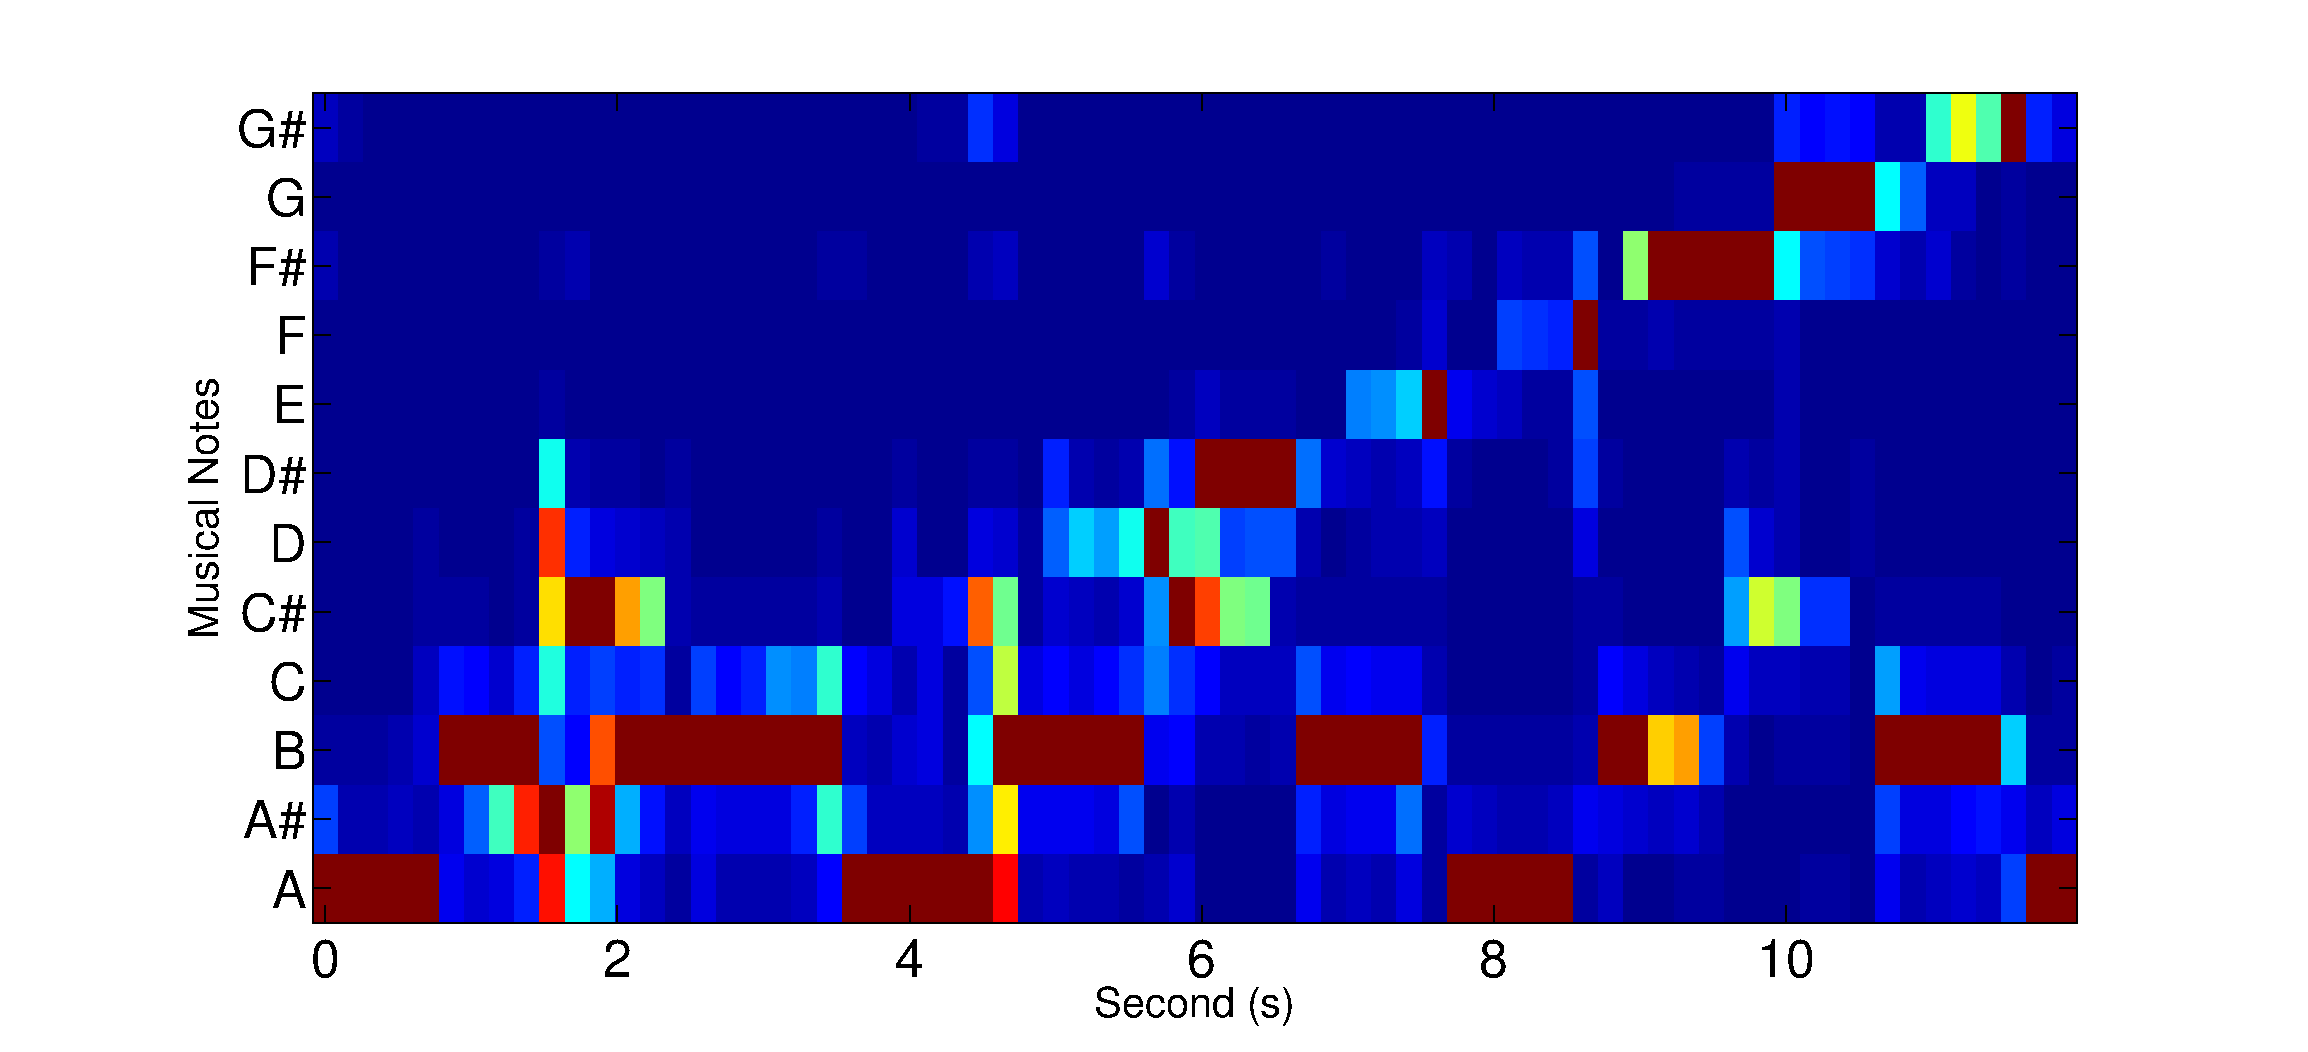
\includegraphics[width=\columnwidth, height=6cm]{figs/2-ccm-violao.eps}}}
	 \caption{Chroma feature of audio using CCM of acoustic guitar tones.}
	 \label{fig:2-ccm-violao}
	\end{figure}	


	\begin{table}[h]
	 \begin{center}
	 \begin{tabular}{|l|l|l|}
	  \hline
	  Piano & Acoustic Guitar & Identified Notes \\
	  \hline
			  A & A &  A \\
		A\# &  B &  B \\
		    A\# &  B &    A\# \\
		    B  &   C\# &  C\# \\
		    C   &  B  &   B \\
		    C\# &  A   &  A \\
		    D   &  B   &  C\# \\
		    D\# &  C\# &  B \\
		    D\# &  C\# &  D \\
		    D\# &  C\# &  C\# \\
		    E   &  B  &   D\# \\
		    F   &  A   &  B \\
		    F   &  A  &   E \\
		    F\# &  B  &   A \\
		    F\# &  B   &  B \\
		    G   &  C\# &  F\# \\
		    G   &  C\# &  C\# \\
		    G\# &  B   &  G \\
		    G\# &  B  &   B \\
	  \hline
	 \end{tabular}
	\end{center}
	 \caption{Comparison between played notes of piano, acoustic guitar and identified notes by the CCM with acoustic guitar tones.}
	 \label{tab:table-2-ccm-violao}
	\end{table}


\section{Discussion}\label{sec:discussion}

	Os resultados alcancados pelo CCM se apresentam mais satisfatorios do que o metodo tradicional STFT, porem com um maior custo computacional agregado aos calculos. O tempo de processamento do metodo da STFT foi de aproximadamente 0.1 segundos contra 13.2 segundos do CCM, no primeiro experimento. Ressalta-se que o elevado custo computacional do CCM nao representa uma limitacao em termos praticos pois o metodo pode ser executado, sem grandes dificuldades, por um computador pessoal.

	No primeiro experimento, o CCM apresentou uma melhora na eficiencia de aproximadamente 28.6\% em relacao ao metodo tradicional STFT. De certa forma o CCM valoriza a energia das notas que tenham correlacao com o sinal de referencia, o que favorece a identificacao. Outro ponto importante eh o fato de o CCM suprimir quais informacoes do sinal que nao estejam correlacionadas com os sinais de referencia utilizados na convolucao. 

	Outro aspecto importante eh a possibilidade, oferecida pelo CCM, de focar a atencao num instrumento especifico a partir da utilizacao de seu timbre, sem custos adicionais para o algoritmo. Notas de referencia gravadas no piano foram melhor identificadas no experimento 2 pois as notas do violao foram suprimidas. O resultado inverso foi observado quando o mesmo sinal de audio foi submetido aos sinais de referencia produzidos pelo violao. A ordem de grandeza das diferencas encontradas para a identificacao das notas privilegiadas pelos sinais de referencia em relacao as notas suprimidas foi da ordem de 40.7\%, em media. O metodo tradicional STFT nao oferece essa possibilidade a menos que otimizacoes sejam praticadas no sentido de considerar o timbre dos instrumentos de uma maneira similar.


	\section{Conclusions and Future Works}\label{sec:conclusions}

	Este trabalho apresentou uma nova forma de contrucao do chroma feature ou PCP, a partir da utilizacao de um novo metodo, aqui denominado por chroma convolution method (CCM). Os resultados obtidos foram confrontados com o algoritmo tradicional STFT revelando uma melhor eficiencia do CCM na identificacao das notas musicais.

	Outra vantagem encontrada para o CCM, em relacao ao metodo tradicional STFT, diz respeito a deteccao de melodias polifonicas, produzidas por mais de um instrumento. O CCM opera com sinais de referencia, para as notas musicais a serem identificadas, que podem ser obtidas de instrumentos reais, fato que, naturalmente, inclui informacoes de timbre na identificacao.

	Este trabalho apresentou uma maneira padrao e basica de utilizacao do CCM, sem quaisquer procedimentos elaborados para reducao de ruido no processo de identificacao das notas. Da mesma forma que o metodo tradicional STFT vem sendo desenvolvido para aplicacoes mais sofisticadas, como o NNLS \cite{mauch2010approximate} e filtro de particulas \cite{jo2010melody}, o metodo CCM pode ser aprimorado para que melhores resultados sejam alcancados.
	
	Vale ressaltar que o CCM e o metodo STFT foram aqui comparados em suas aplicacoes basicas, ou seja, muito se tem para fazer em relacao a aplicacao do CCM sobre a identificacao de acordes e melodias polifonicas, considerando o grande volume e a qualidade dos trabalhos ja produzidos pelas solucoes tradicionais no dominio da frequencia.	


% For bibtex users:
\bibliography{ISMIR2015template}

% For non bibtex users:
%\begin{thebibliography}{citations}
%
%\bibitem {Author:00}
%E. Author.
%``The Title of the Conference Paper,''
%{\it Proceedings of the International Symposium
%on Music Information Retrieval}, pp.~000--111, 2000.
%
%\bibitem{Someone:10}
%A. Someone, B. Someone, and C. Someone.
%``The Title of the Journal Paper,''
%{\it Journal of New Music Research},
%Vol.~A, No.~B, pp.~111--222, 2010.
%
%\bibitem{Someone:04} X. Someone and Y. Someone. {\it Title of the Book},
%    Editorial Acme, Porto, 2012.
%
%\end{thebibliography}

\end{document}
